\section{联邦学习算法整体效果的数值评测}
\addcontentsline{toe}{section}{{\thesection\ \ Numerical Evaluation of the Overall Effectiveness of Federated Learning Algorithms}\numberline\,}
% \esection{Numerical Evaluation of the Overall Effectiveness of Federated Learning Algorithms}
\label{sec:chap6-overall}

% almost finished

本节对几种典型的联邦学习算法进行数值上的评测,包括
\begin{itemize}
    \item \texttt{FedAvg}\cite{mcmahan2017fed_avg} (作为\texttt{FedOpt}\cite{reddi2020fed_opt}的特例),
    \item \texttt{FedAdam}\cite{reddi2020fed_opt, adam} (作为\texttt{FedOpt}\cite{reddi2020fed_opt}的特例),
    \item \texttt{FedAdagrad}\cite{reddi2020fed_opt, adagrad} (作为\texttt{FedOpt}\cite{reddi2020fed_opt}的特例),
    \item \texttt{FedYogi}\cite{reddi2020fed_opt, Zaheer_2018_yogi} (作为\texttt{FedOpt}\cite{reddi2020fed_opt}的特例),
    \item \texttt{FedProx}\cite{sahu2018fedprox},
    \item \texttt{Ditto}\cite{li_2021_ditto},
    \item \texttt{FedSplit}\cite{pathak2020fedsplit},
    \item \texttt{IFCA}\cite{Ghosh_2022_cfl},
    \item \texttt{ProxSkip}\cite{proxskip},
    \item \texttt{SCAFFOLD}\cite{karimireddy2020scaffold}.
\end{itemize}
各个算法的超参数的设置基本与本报告\S\ref{sec:chap5-design}中展示的典型的联邦学习仿真系统\texttt{fl-sim}命令行接口配置文件\ref{lst:fl-sim-config}~一致,即整体进行100轮次的迭代循环;在每一轮循环内,子节点以步长0.03执行10步子问题迭代训练,训练数据的批大小 (Batch Size)\index{批大小, Batch Size} 采用数据集\texttt{FedProxFEMNIST}预置的默认批大小,值为20.

图\ref{fig:standard-test-ratio-10-val-acc}~是以上列出的几种联邦学习优化算法在在子节点训练参与率为$10\%$ (或者等价地,子节点掉队 (Straggler) 几率为$90\%$) 的场景下,在数据集\texttt{FedProxFEMNIST}的测试集上的准确率曲线。可以看到\texttt{FedOpt}相关的几种算法:\texttt{FedAdam}, \texttt{FedAdagrad}, \texttt{FedYogi}, 包括\texttt{FedAvg},在这种比较极端的场景下,都有非常不错的鲁棒性。除此之外,\texttt{IFCA}, \texttt{Ditto}等算法在这种场景下的鲁棒性也不错。而联邦临近算法\texttt{FedProx}在这种场景下的模型准确率曲线波动比较剧烈,而且在整体100轮的迭代之后还未收敛。\texttt{ProxSkip}以及\texttt{FedSplit}算法在子节点训练参与率为$10\%$的场景下发散。

\begin{figure}[H]
    \centering
    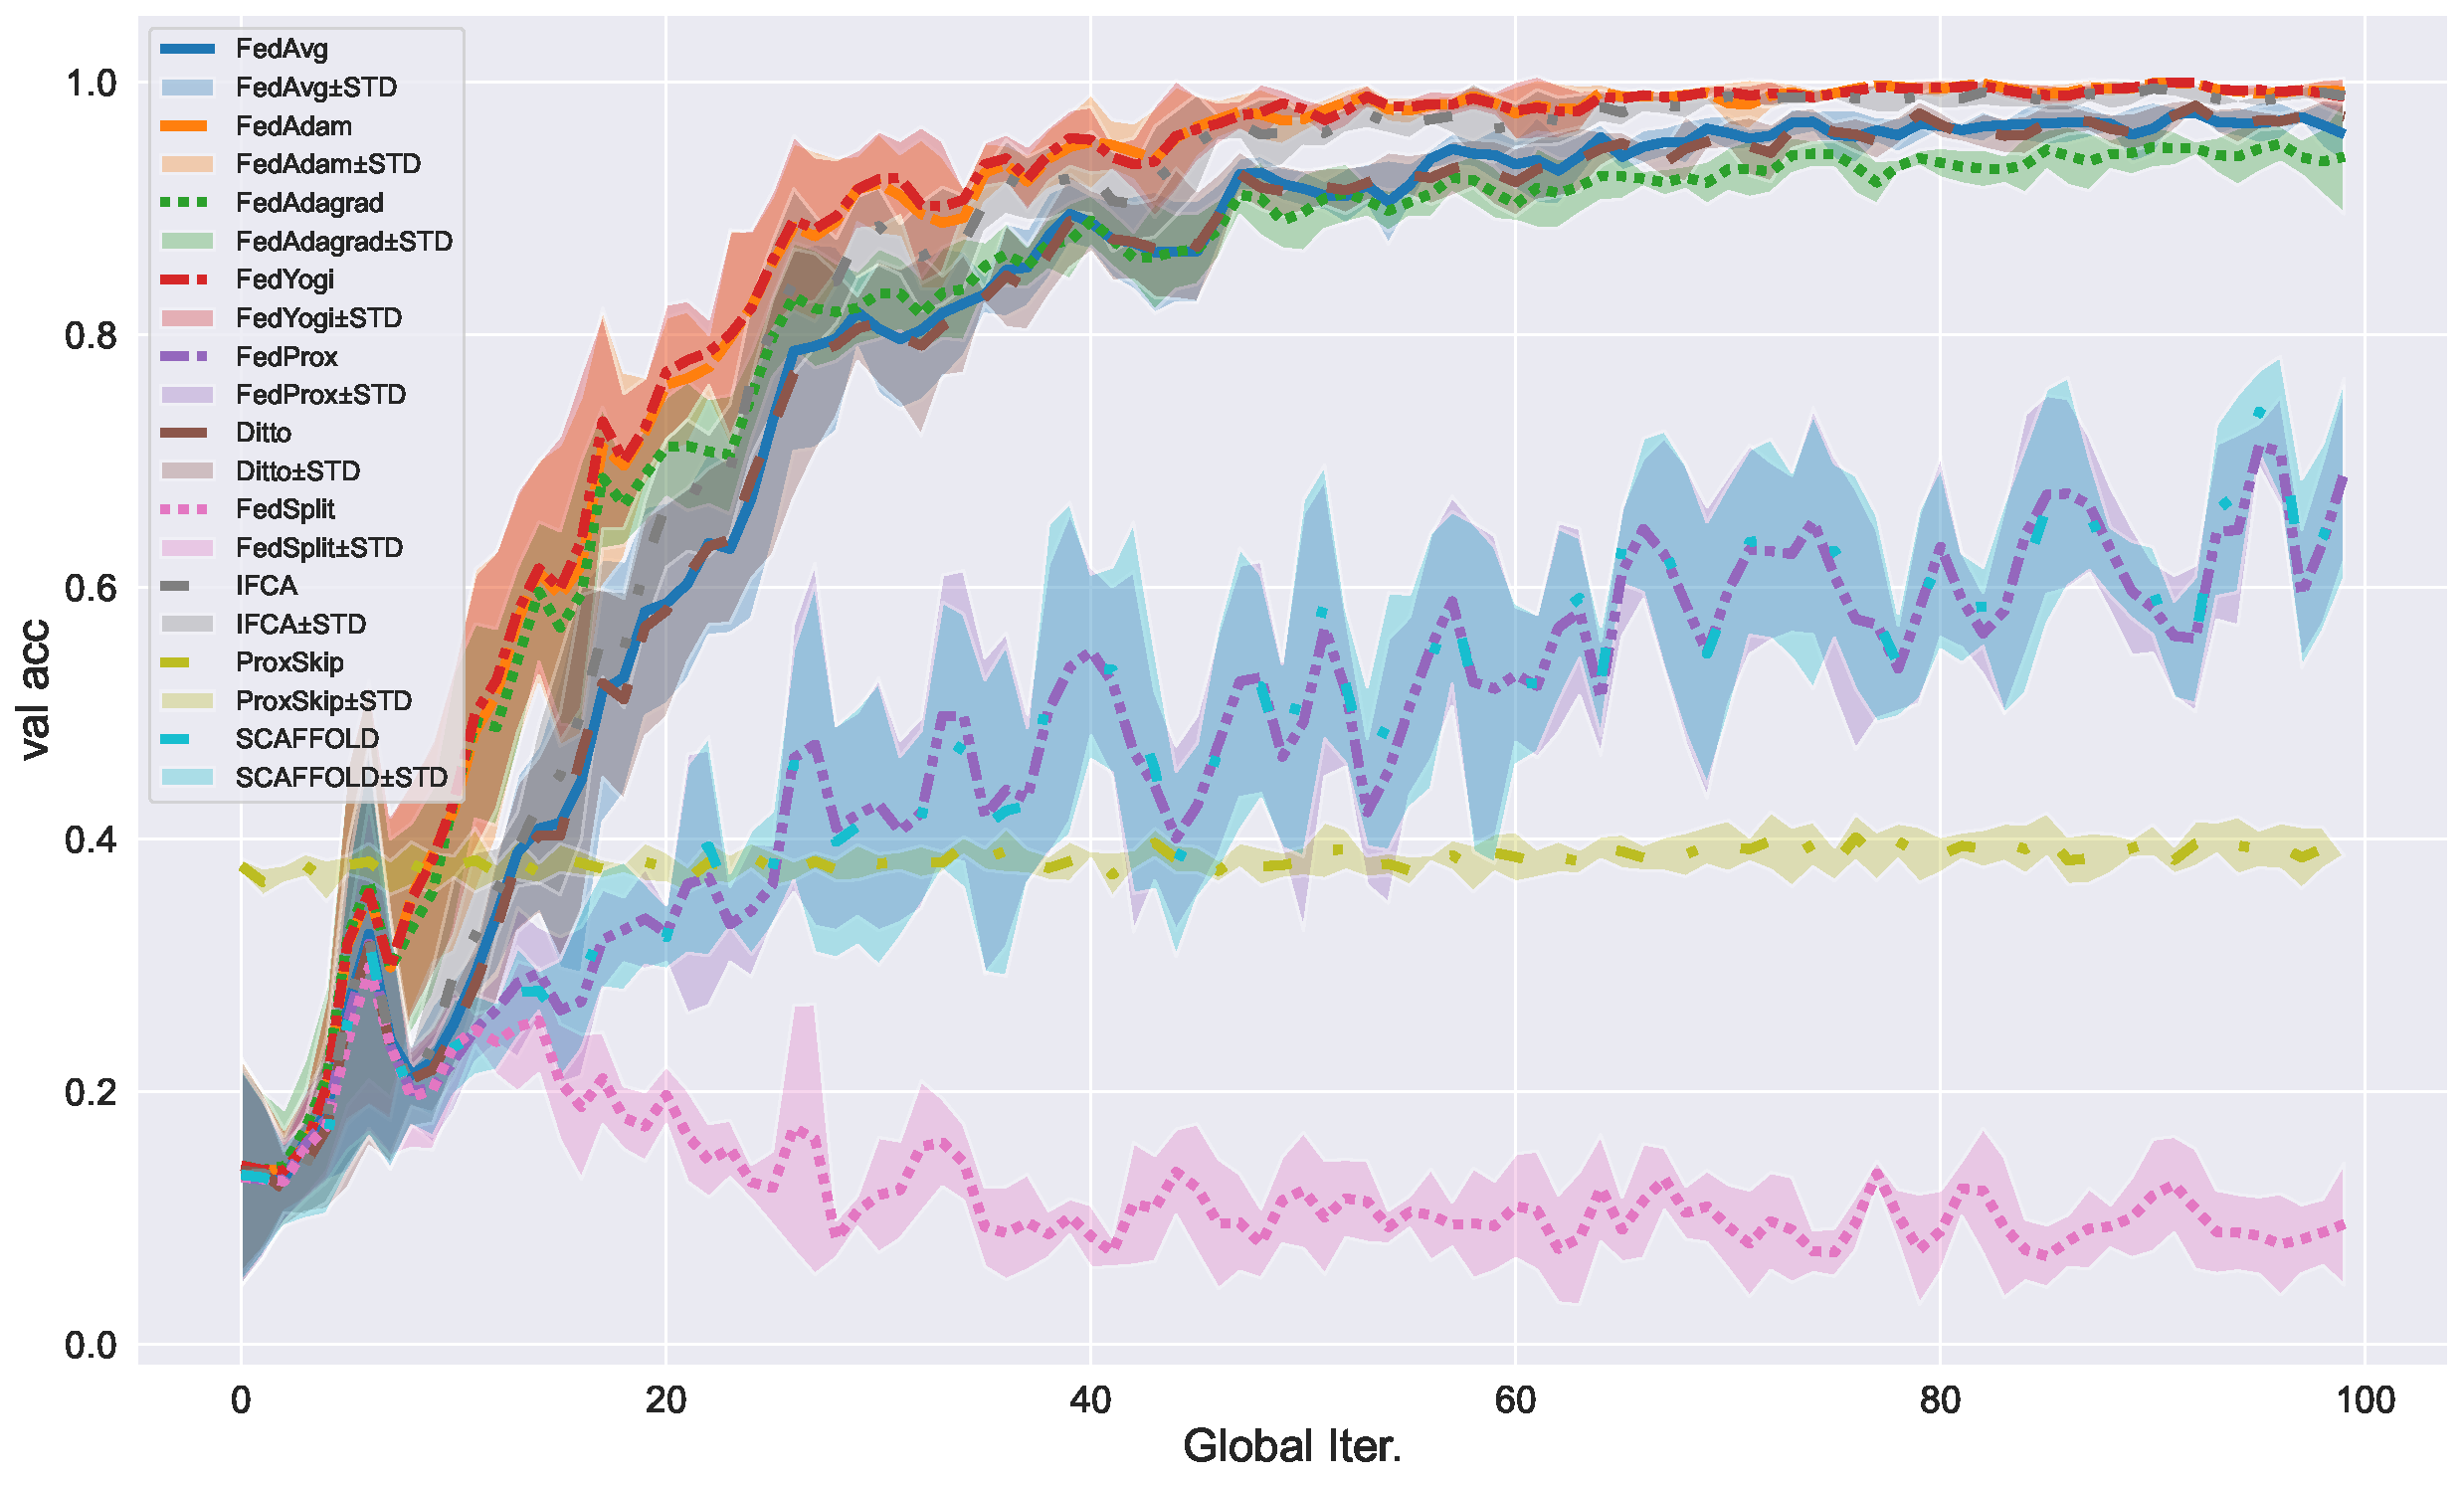
\includegraphics[width=0.9\textwidth]{figures/standard-test-ratio-10-val-acc.pdf}
    \caption{几种典型的联邦学习算法在子节点训练参与率为$10\%$时,在测试集上的准确率曲线}
    \label{fig:standard-test-ratio-10-val-acc}
\end{figure}

图\ref{fig:standard-test-ratio-30-val-acc}, \ref{fig:standard-test-ratio-70-val-acc}, \ref{fig:standard-test-ratio-100-val-acc}~分别是这几种联邦学习优化算法在在子节点训练参与率为$30\%,$ $70\%,$ 以及$100\%$时,在数据集\texttt{FedProxFEMNIST}的测试集上的准确率曲线。可以看到,随着每轮参与训练的子节点比例的提升,或者等价地,每一轮子节点掉队比例的降低,包括\texttt{FedProx}, \texttt{ProxSkip}在内的联邦学习优化算法的稳定性是逐渐提升的,而这其中\texttt{ProxSkip}算法受到的影响是更大的。对于联邦分裂算法\texttt{FedSplit}来说,只有当子节点训练参与率为$100\%$时才不发散,而且在这种情况下,其收敛速度也较慢。

\begin{figure}[H]
    \centering
    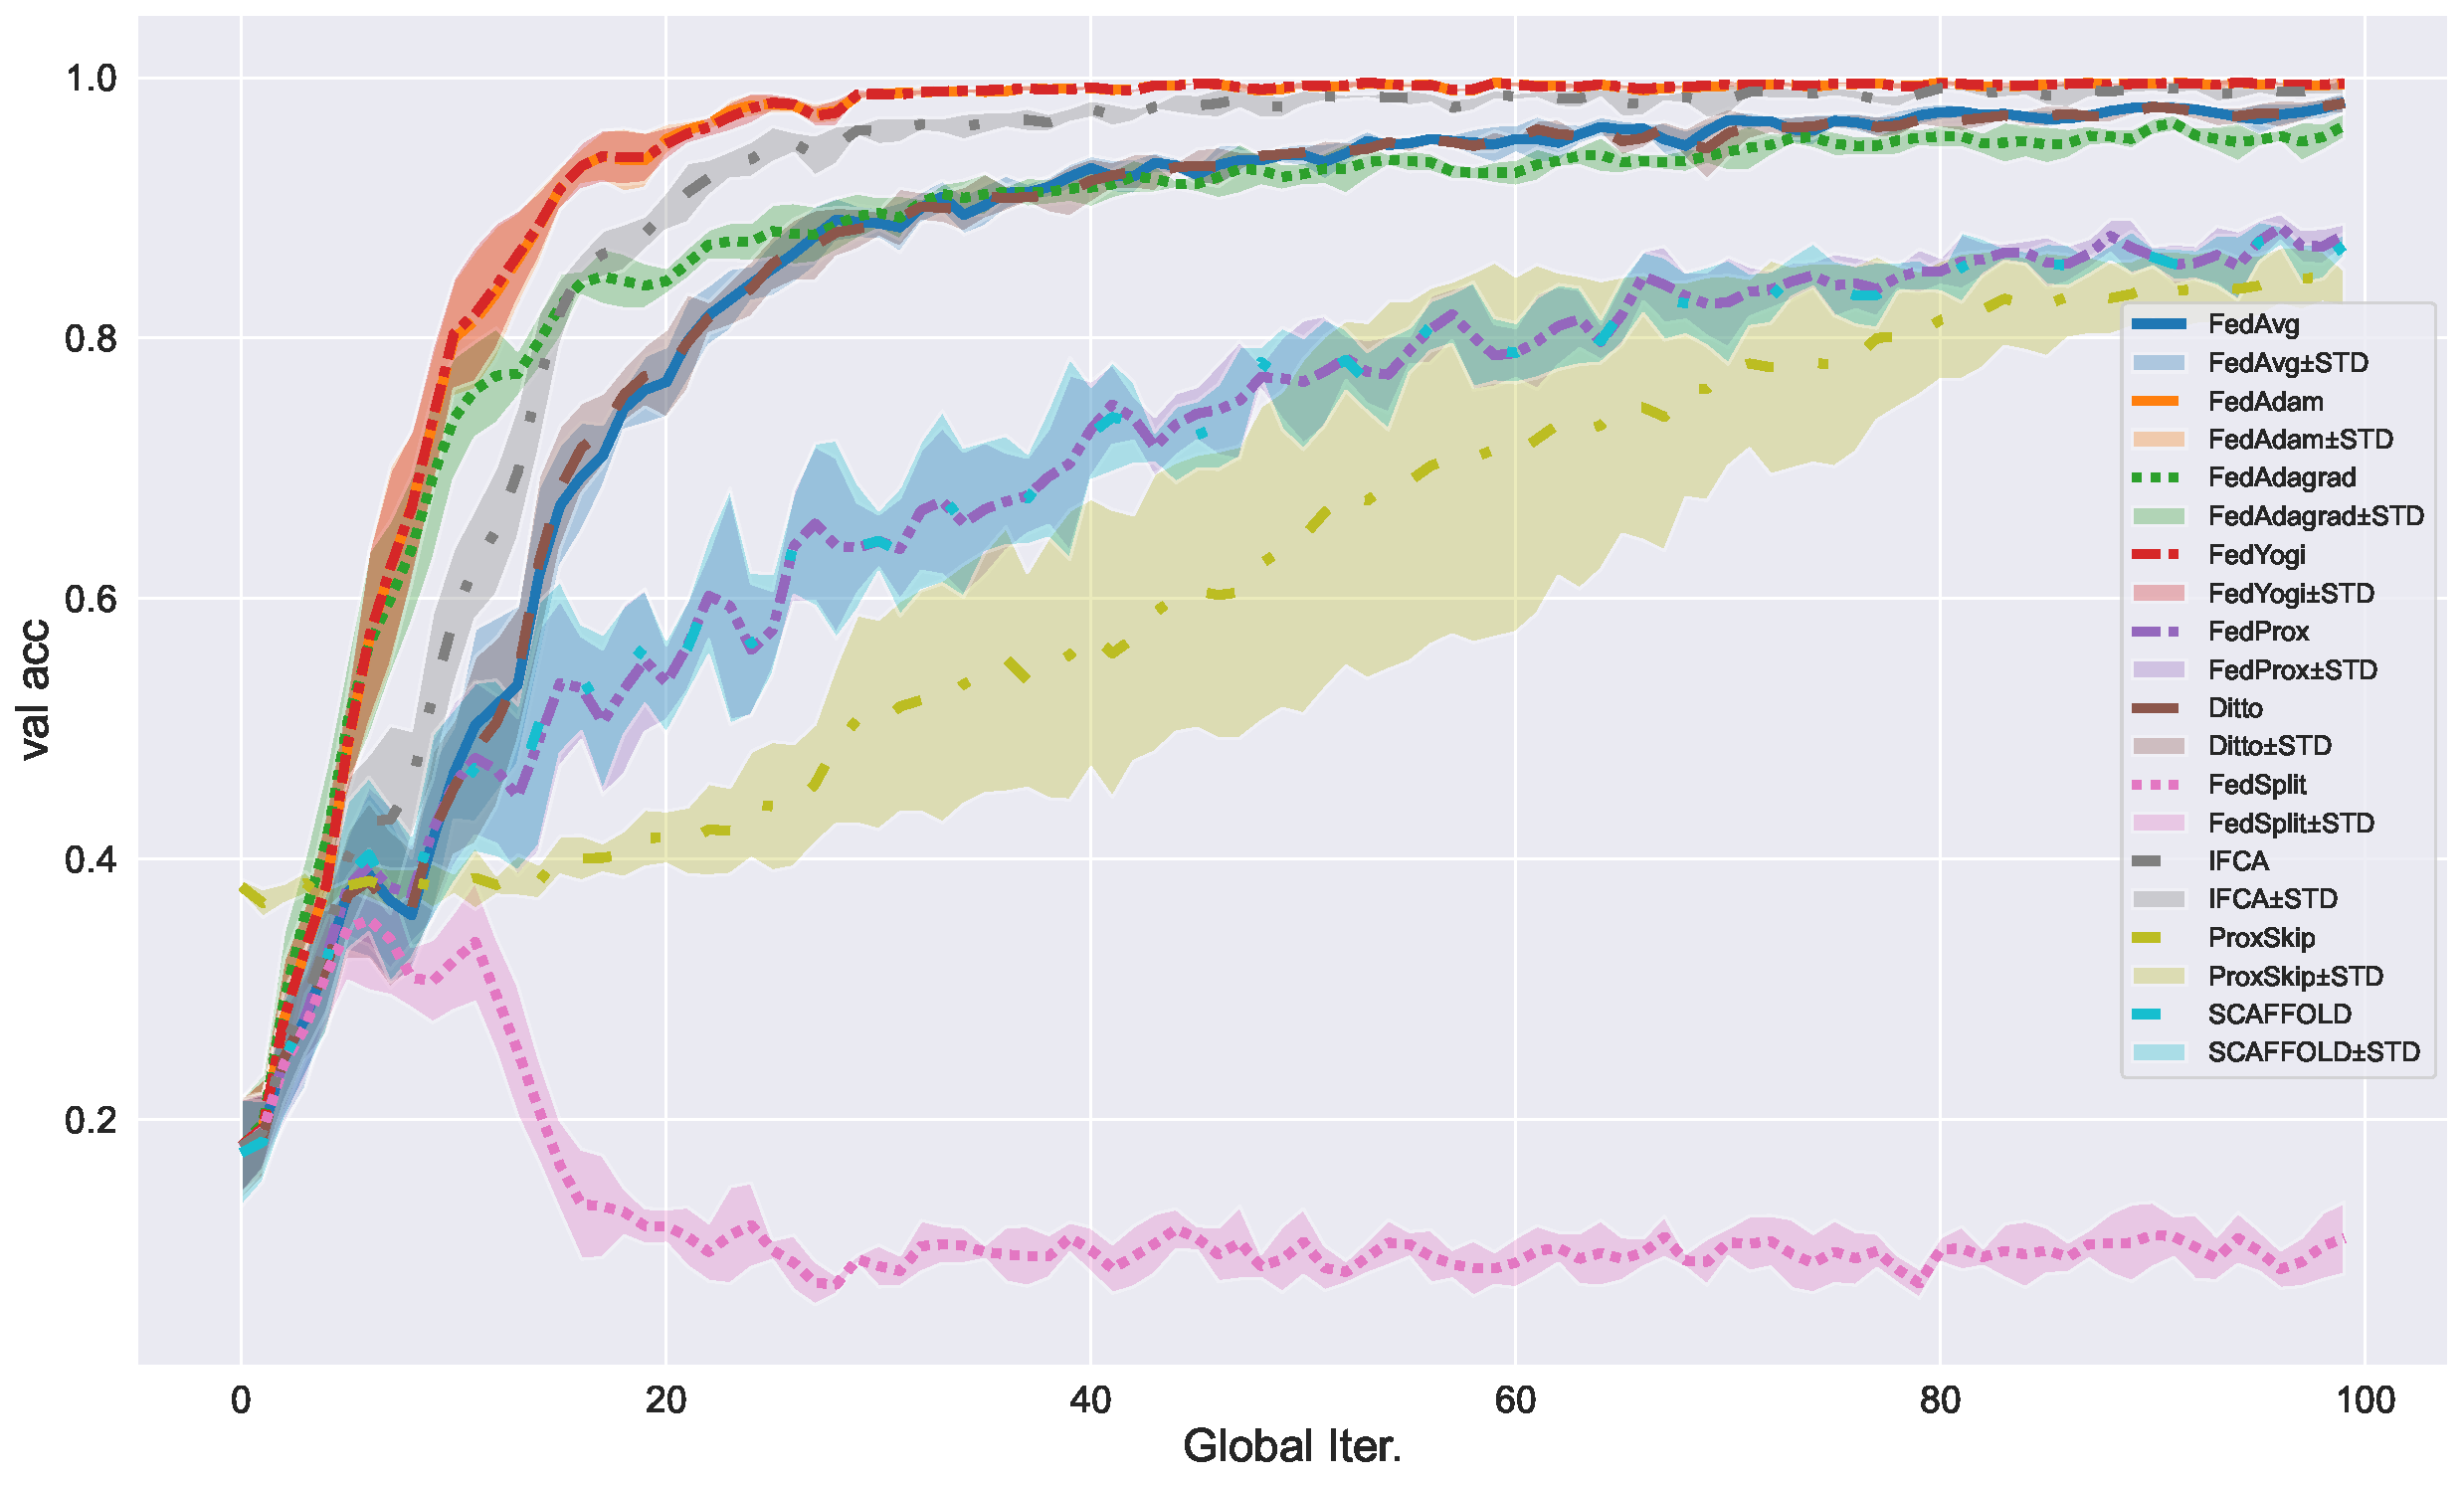
\includegraphics[width=0.9\textwidth]{figures/standard-test-ratio-30-val-acc.pdf}
    \caption{几种典型的联邦学习算法在子节点训练参与率为$30\%$时,在测试集上的准确率曲线}
    \label{fig:standard-test-ratio-30-val-acc}
\end{figure}

\begin{figure}[H]
    \centering
    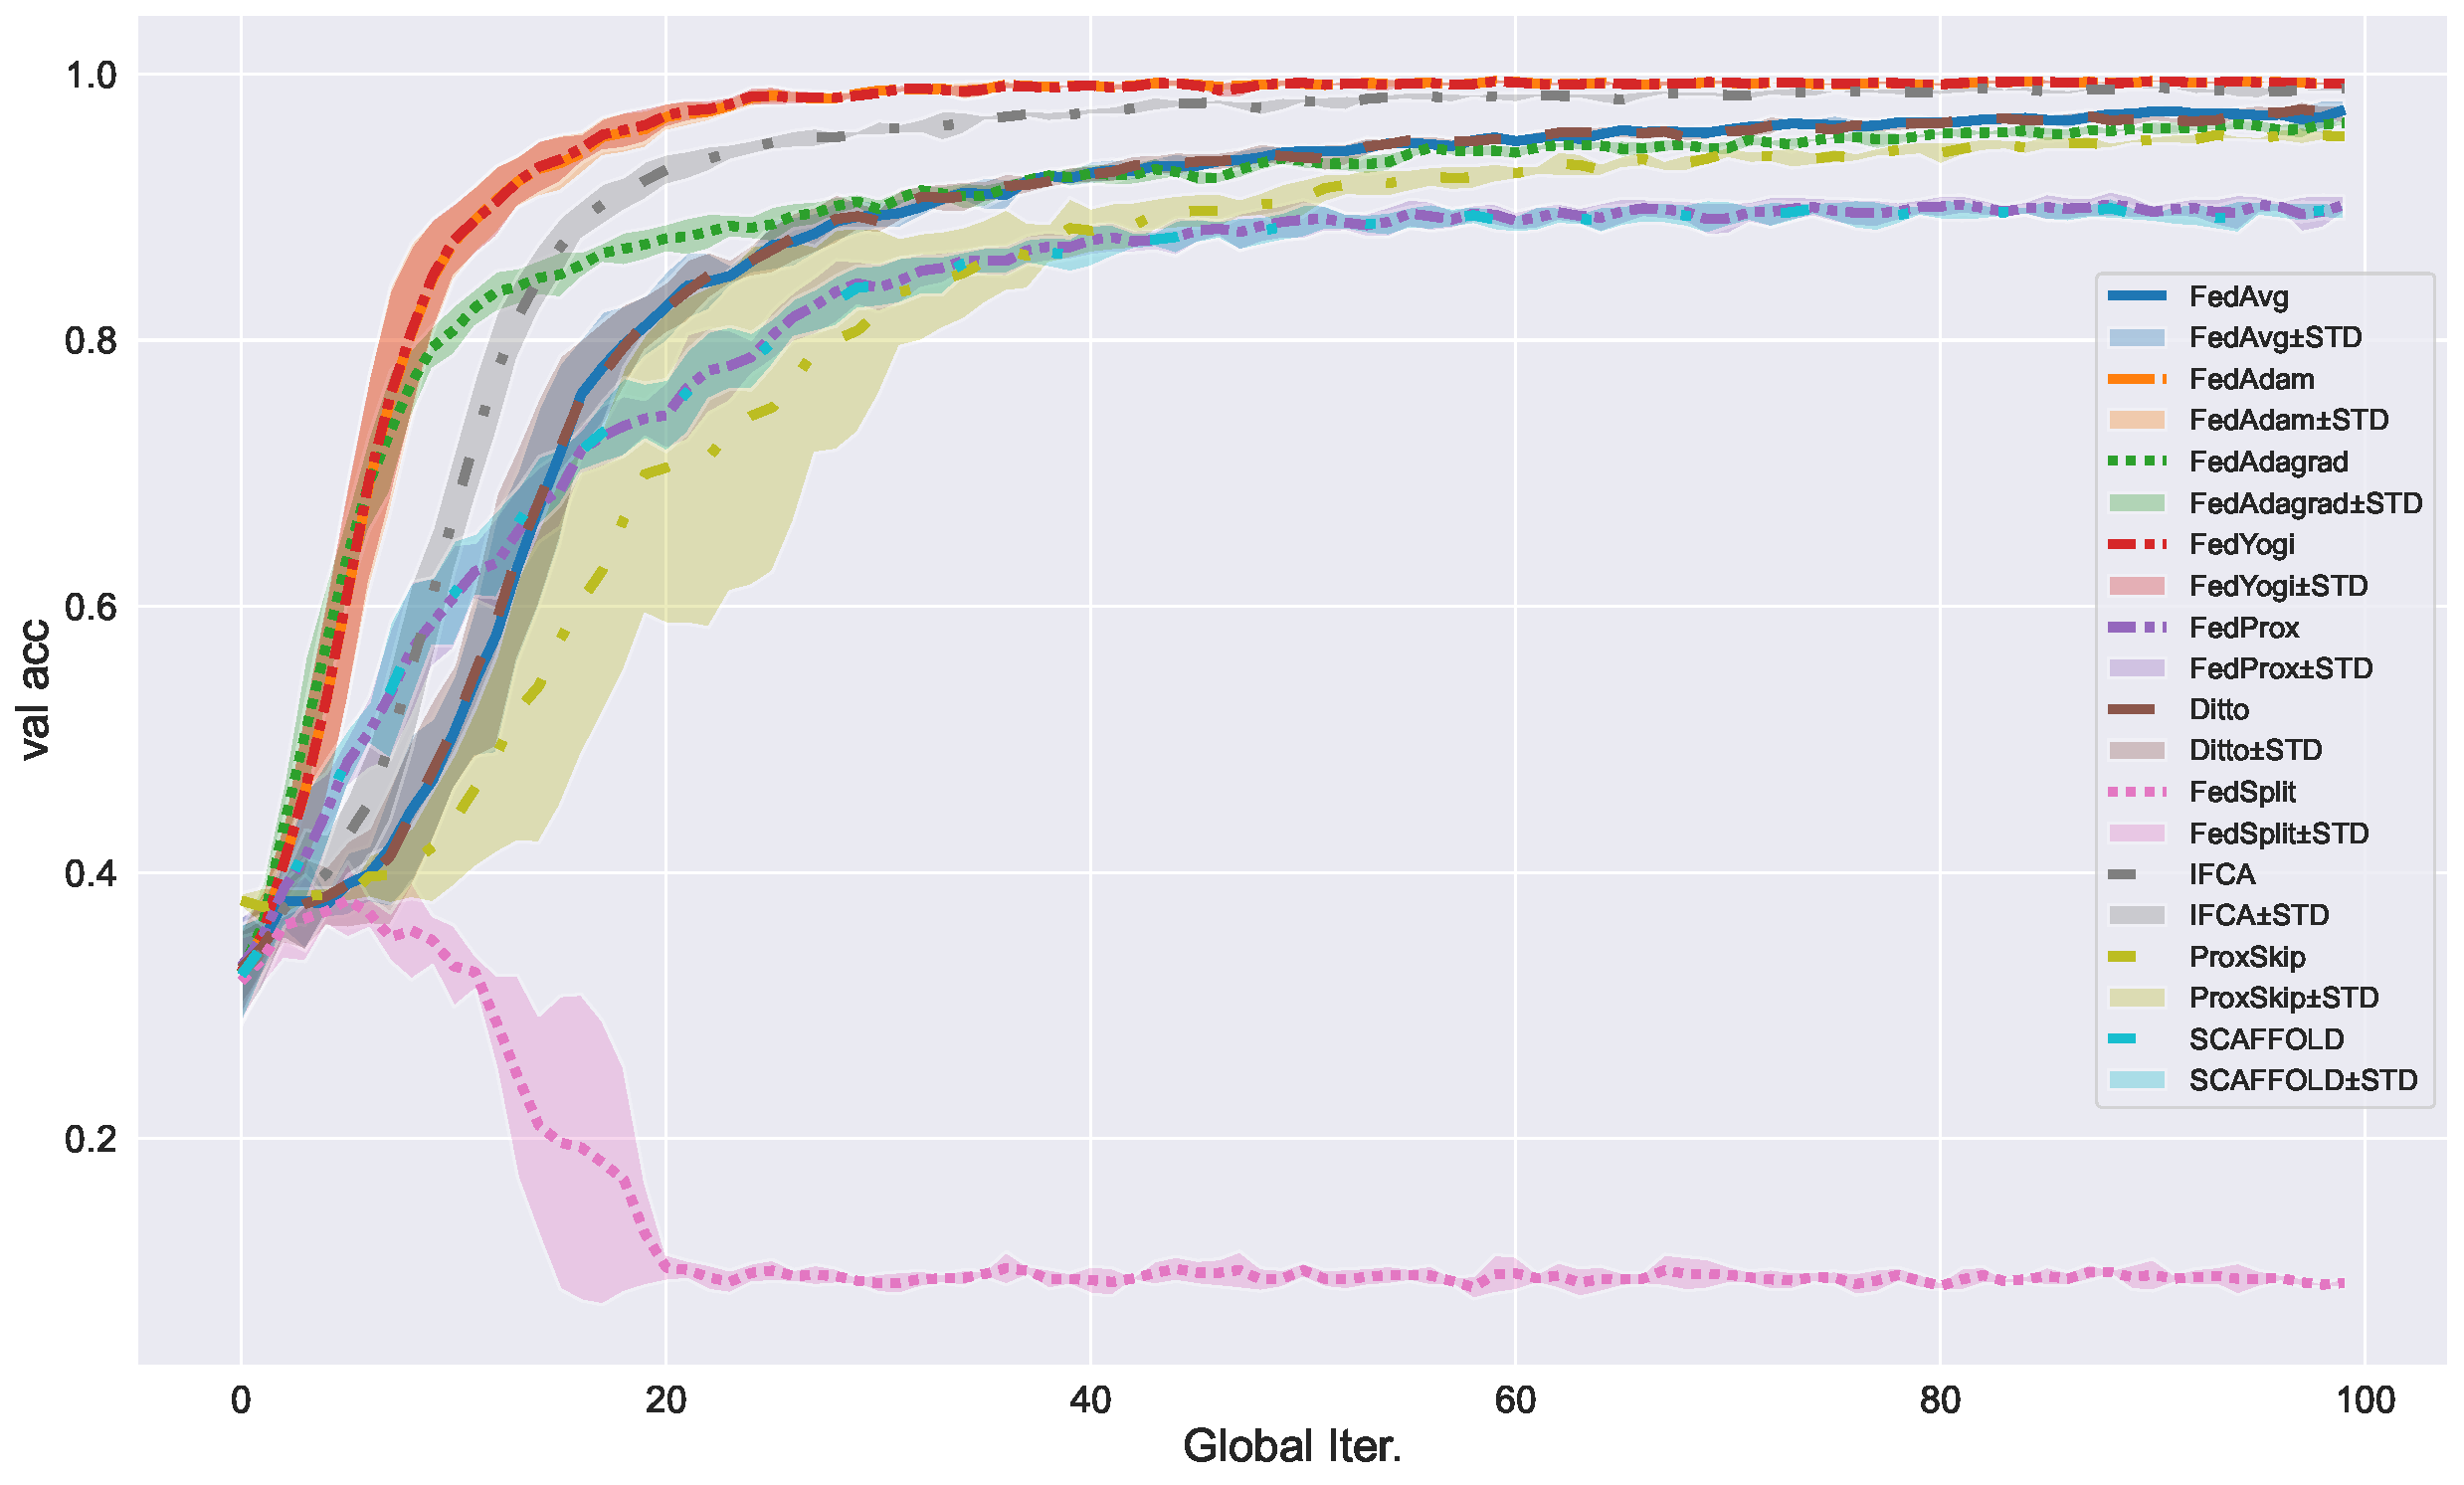
\includegraphics[width=0.9\textwidth]{figures/standard-test-ratio-70-val-acc.pdf}
    \caption{几种典型的联邦学习算法在子节点训练参与率为$70\%$时,在测试集上的准确率曲线}
    \label{fig:standard-test-ratio-70-val-acc}
\end{figure}

\begin{figure}[ht]
    \centering
    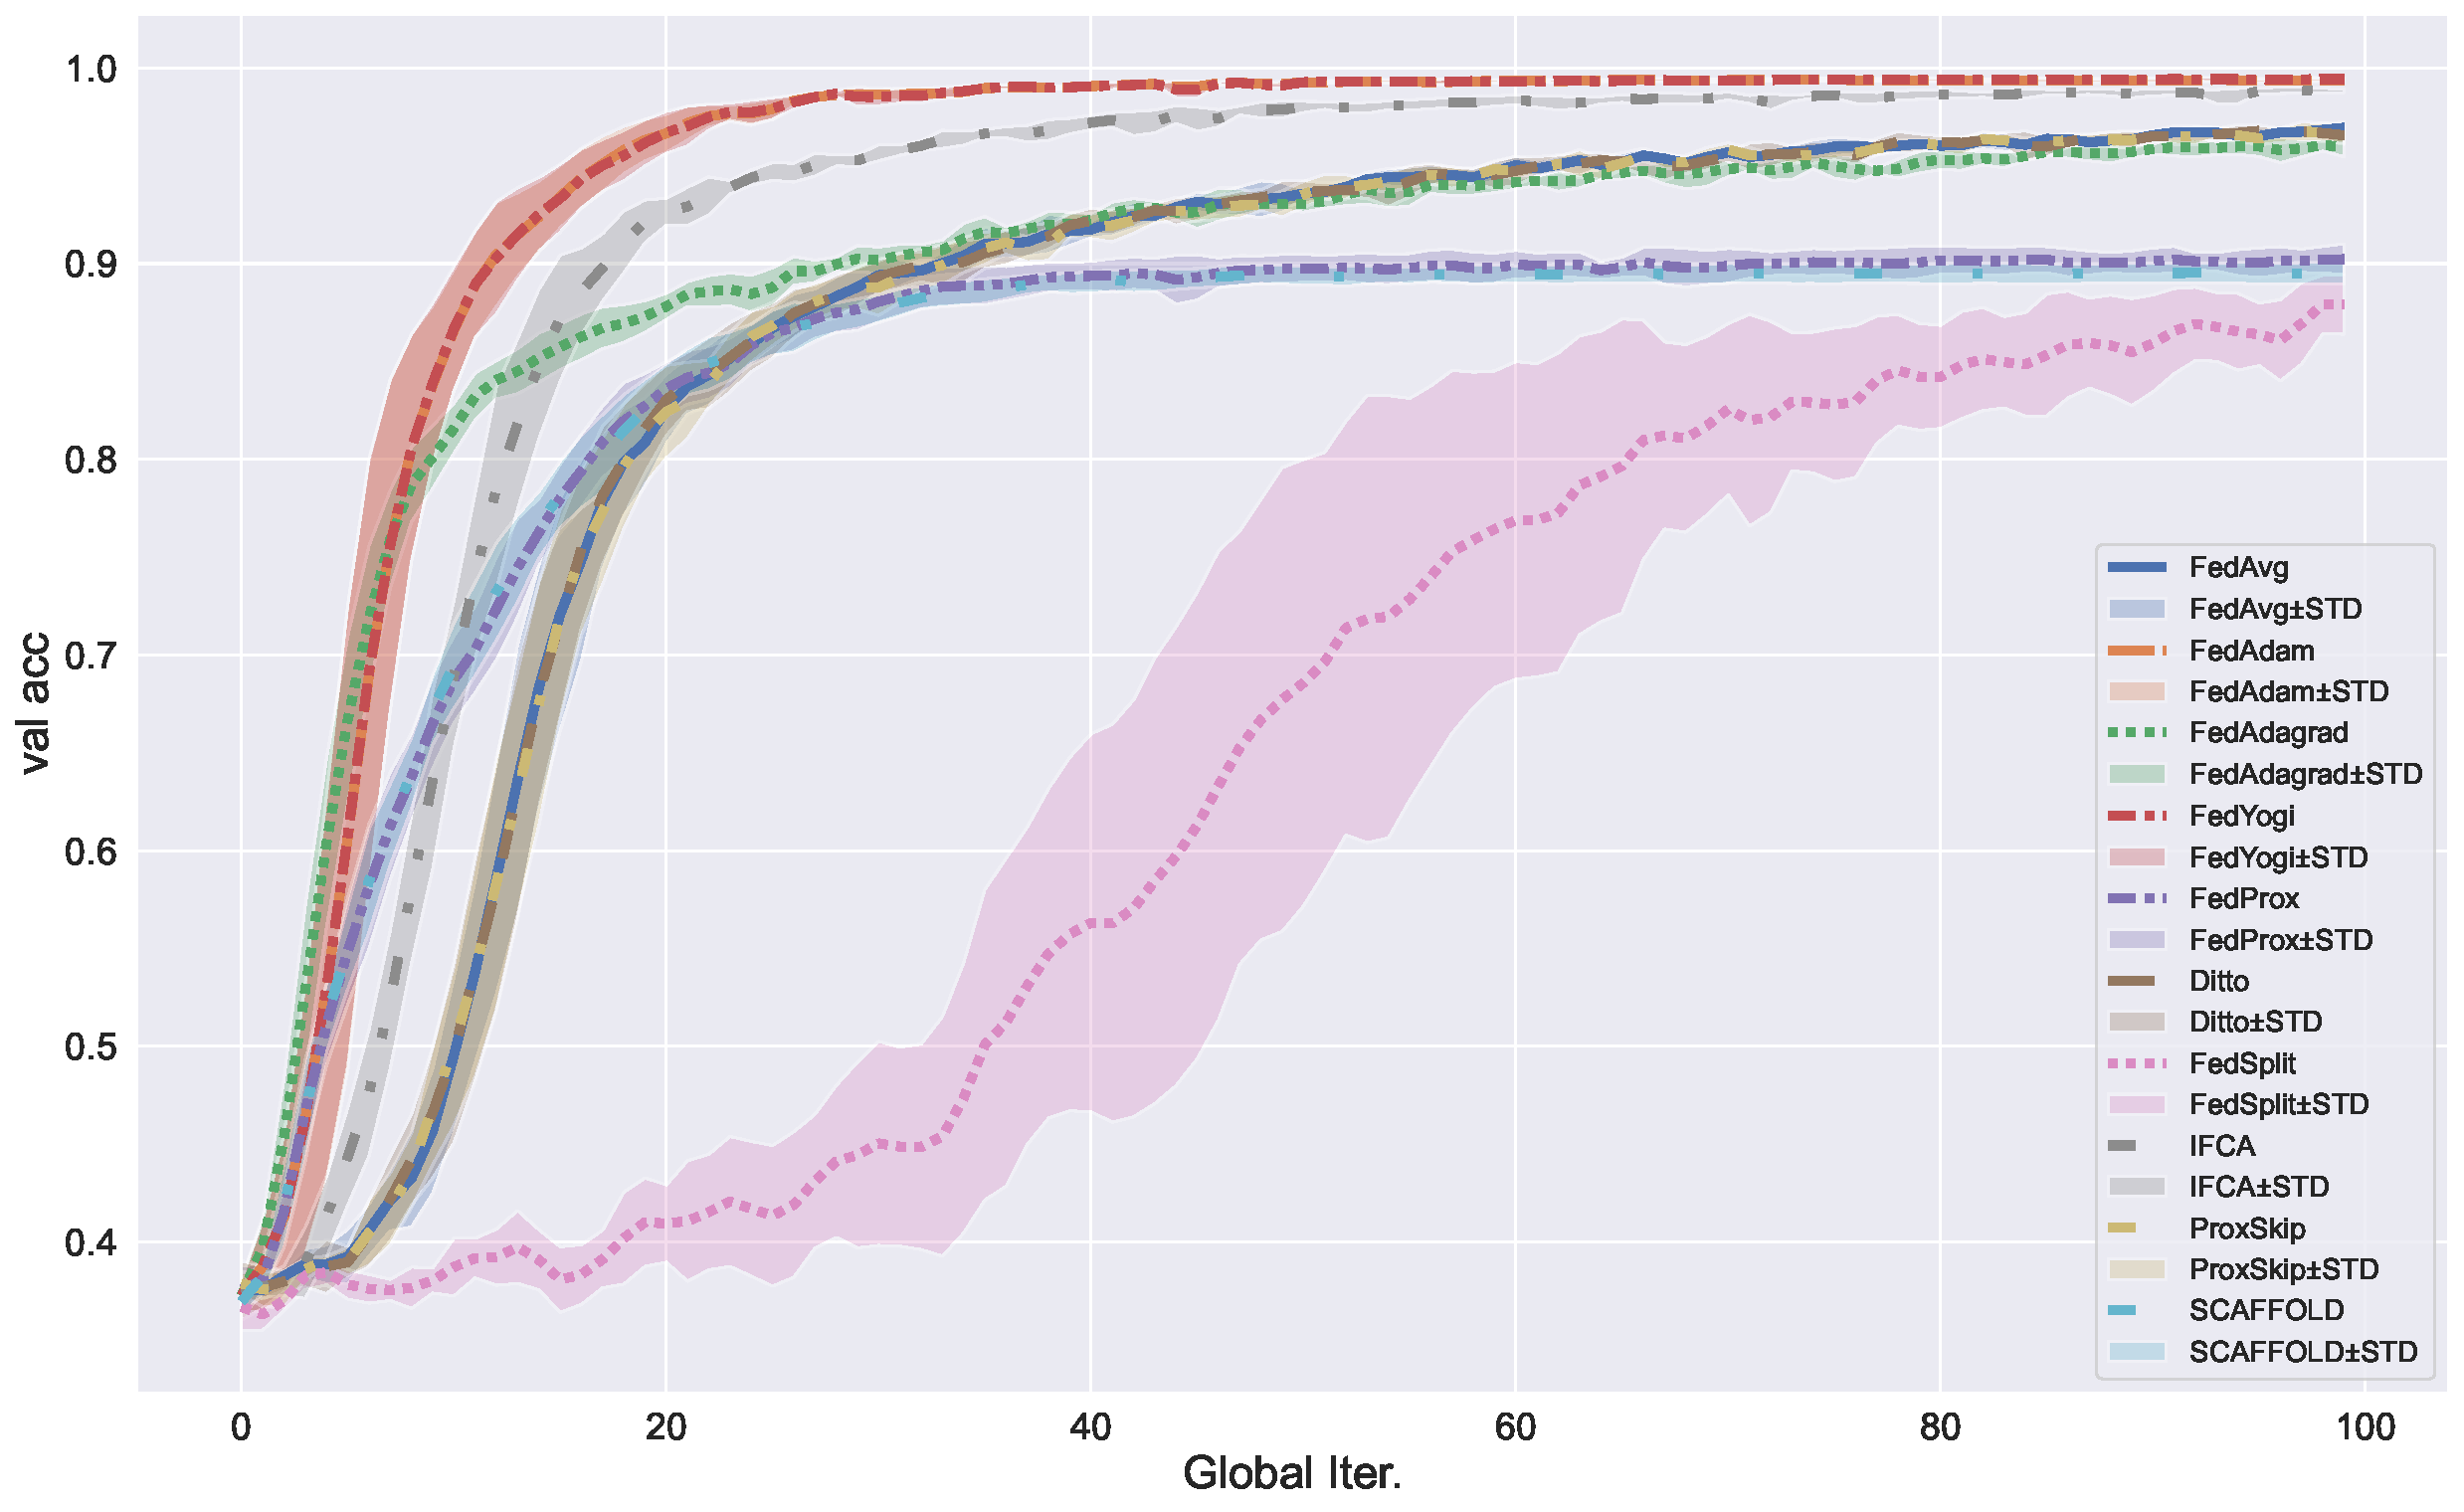
\includegraphics[width=0.9\textwidth]{figures/standard-test-ratio-100-val-acc.pdf}%to upload
    \caption{几种典型的联邦学习算法在子节点训练参与率为$100\%$时,在测试集上的准确率曲线}
    \label{fig:standard-test-ratio-100-val-acc}
\end{figure}

通过这一组数值实验,可以看到,\texttt{FedAdam}, \texttt{FedYogi}算法在设置了合适的全局步长 (关于相关算法全局步长的讨论,详见本章\S\ref{sec:chap6-lr}以及参考文献\parencite{reddi2020fed_opt}附录D.4) 的前提下,在收敛速度、算法效果 (以测试集上准确率计) 、稳定性以及关于子节点参与每轮训练比例的鲁棒性等方面都是十分出色的。有聚类数目先验知识的聚类联邦算法\texttt{IFCA} (注意到在配置文件\ref{lst:fl-sim-config}~中,我们为\texttt{IFCA}算法设置的聚类数目与数据集\texttt{FedProxFEMNIST}天然具有的聚类结构是相匹配的) 在这些方面表现稍次之。在收敛速度、算法效果、稳定性、鲁棒性等方面再次一些的是\texttt{FedAvg}, \texttt{FedAdagrad}, \texttt{Ditto}等算法. 自适应联邦算法\texttt{FedAdam}, \texttt{FedYogi}, \texttt{FedAdagrad}, 以及联邦平均算法\texttt{FedAvg}这几个算法之间的数值比较关系基本与参考文献\parencite{reddi2020fed_opt}第4节以及第5节进行的数值实验结果相符。

\texttt{FedProx}, \texttt{ProxSkip}等算法在收敛速度、算法效果、稳定性、鲁棒性等某些方面与上述算法有一定的差距,特别是关于子节点参与每轮训练比例的鲁棒性等方面。另一个指的关注的问题是,当子节点训练参与率为$100\%$时,跳步算法\texttt{ProxSkip}实际上就是联邦平均算法\texttt{FedAvg},这一点可以从图\ref{fig:standard-test-ratio-100-val-acc}看出。但是当子节点训练参与率低于$100\%$时,跳步算法\texttt{ProxSkip}的鲁棒性明显比联邦平均算法\texttt{FedAvg}低。二者的区别在于,例如当子节点训练参与率等于$30\%$时,跳步算法\texttt{ProxSkip}约定在比例为$30\%$的训练轮次进行子节点与中心节点的通信与全局模型的更新,而在其余训练轮次,所有子节点只进行本地训练,并不与中心节点通信、更新全局模型。联邦平均算法\texttt{FedAvg}则是在每一个训练轮次选取$30\%$的子节点与中心节点通信,利用这部分信息更新全局模型。后者的做法更符合实际的联邦学习场景,并且从数值上看也更加鲁棒。

对于联邦分裂算法\texttt{FedSplit}来说,只有子节点训练参与率达到$100\%$的时候,算法才能收敛。可以从算法伪代码\ref{algo:fedsplit}看到,它并没有考虑每轮迭代只有部分子节点参与的情况,这也是基于算子分裂方法设计的联邦学习算法需要注意的潜在问题。同时可以看到的是,联邦分裂算法\texttt{FedSplit}收敛速度较慢,且到100轮迭代仍未收敛。针对这一问题,我们执行了另一组数值实验,将全局迭代轮数从100提升到200,并保持其余参数参数不变,相关的测试集上的准确率曲线以及损失曲线绘制在图\ref{fig:fedsplit-200}~中。可以看到,在全局100轮迭代之后,联邦分裂算法\texttt{FedSplit}逐渐开始收敛,但到200轮之后,仍未完全收敛。

\begin{figure}[ht]
\centering
\begin{subfigure}{.7\textwidth}
  \centering
  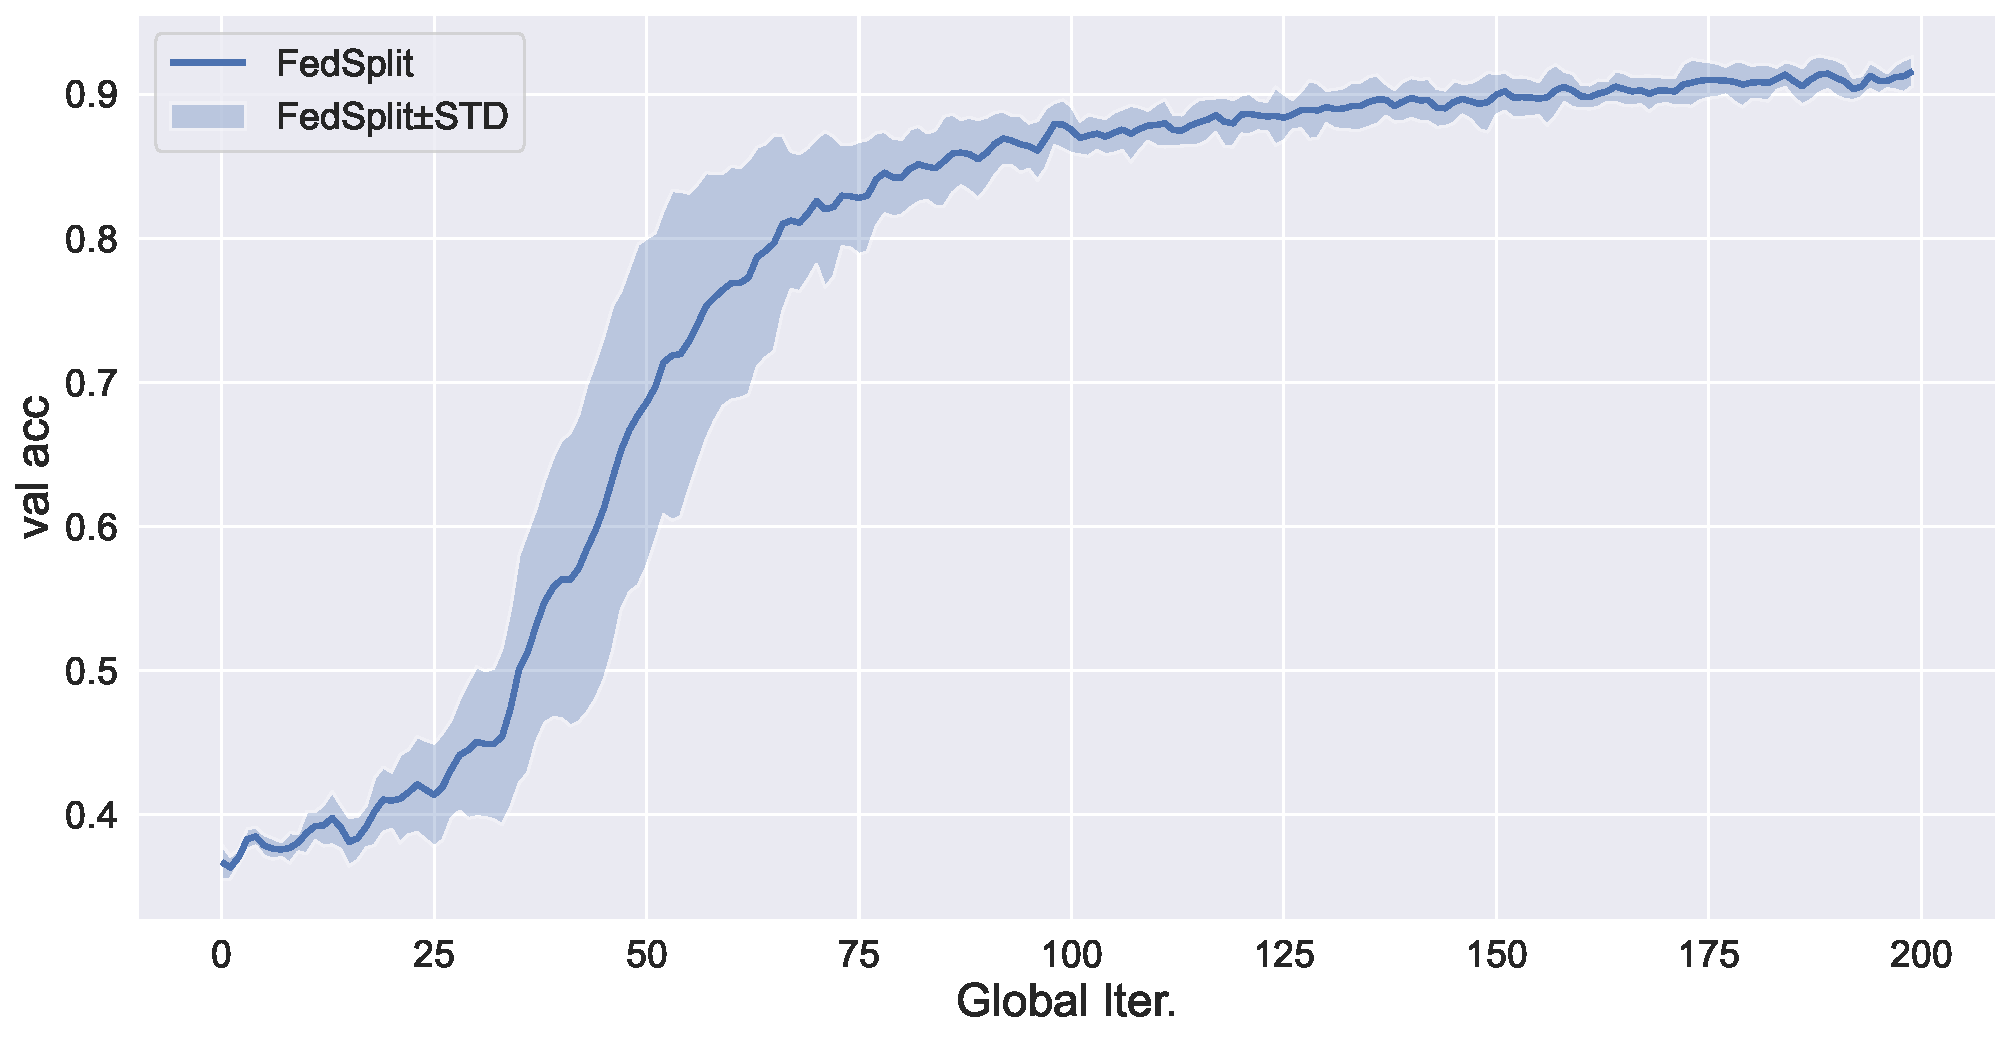
\includegraphics[width=.95\linewidth]{figures/fedsplit-200-val-acc.pdf}
  \caption{\texttt{FedSplit}算法在测试集上准确率曲线}
  \label{fig:fedsplit-200-val-acc}
\end{subfigure}
\begin{subfigure}{.7\textwidth}
  \centering
  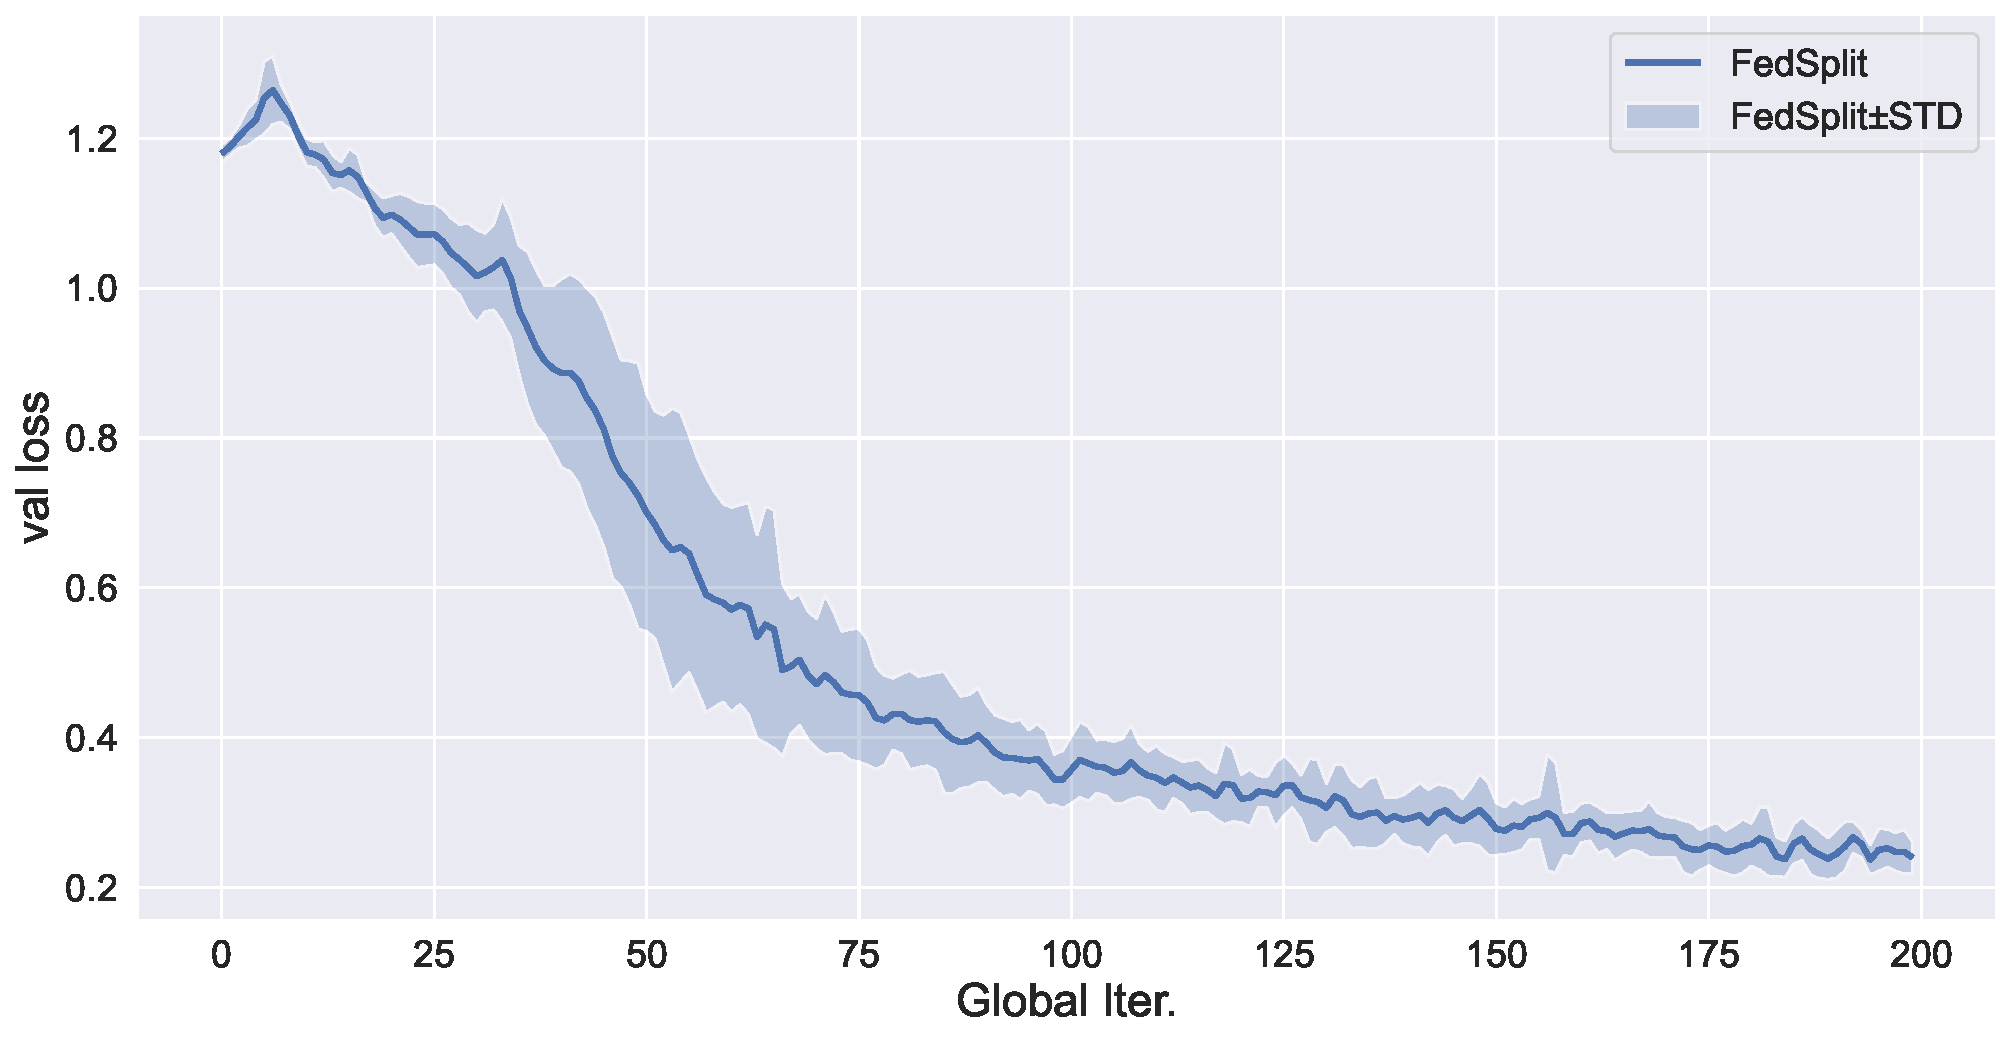
\includegraphics[width=.95\linewidth]{figures/fedsplit-200-val-loss.pdf}
  \caption{\texttt{FedSplit}算法在测试集上损失曲线}
  \label{fig:fedsplit-200-val-loss}
\end{subfigure}
\caption{联邦分裂算法\texttt{FedSplit}在子节点训练参与率为$100\%$下以及全局迭代轮数$200$下,在数据集\texttt{FedProxFEMNIST}的测试集上的准确率曲线以及损失曲线。}
\label{fig:fedsplit-200}
\end{figure}
